\documentclass[a4paper,10pt,oneside,openany]{book}

\usepackage[english]{babel}

\usepackage[utf8]{inputenc} % Consente l'uso dei caratteri accentati italiani
\usepackage[T1]{fontenc} % Consente l'uso di caratteri speciali appartenenti in genere ad alfabeti non inglesi

\usepackage{fancyhdr} % Consente il rendering della copertina

\usepackage{graphicx} % Consente l'inserimento delle figure nel documento

\usepackage{subfigure} % Consente l'inserimento di sottofigure

\usepackage{tabularx} % Consente l'uso di funzionalità aggiuntive alle tabelle
\usepackage{longtable} % Consente la scrittura delle tabelle su più pagine

\usepackage[titletoc]{appendix} % Consente di porre le appendici in indice

\usepackage{float} % Necessario per inserire immagini flottanti

\usepackage{fancyvrb} % Consente l'utilizzo di finestre Verbatim (testo cche si vuole porre così com'è, senza formattazione alcuna) all'interno di una cornice

\usepackage{amsmath} % Consente l'uso di funzioni aggiuntive per le formule
\numberwithin{equation}{section}

\usepackage{hyperref} % Indice degli argomenti e rimandi cliccabili, per una navigazione più comoda all'interno del file

\usepackage{lipsum} % Consente di inserire testo fittizio all'interno della tesi. Inutile in fase di scrittura della tesi. Eliminare questa dicitura e tutte le diciture \lorem all'interno del testo.

\usepackage{rotating} % to rotate images


\usepackage{lineno}
\modulolinenumbers[1]

\usepackage[nopostdot,style=super,nonumberlist,toc, automake]{glossaries}
\makeglossaries
\renewcommand{\glossarysection}[2][]{}


\setacronymstyle{long-short}
\newacronym{clup}{CLup}{Customers Line-up}
\newacronym{dpcm}{d.P.C.m}{\textit{"decreto del Presidente del Consiglio dei ministri"}}
\newacronym{gps}{GPS}{Global Positioning System}
\newacronym{fifo}{FIFO}{First In First Out}
\newacronym{api}{API}{Application Programming Interface}
\newacronym{uml}{UML}{Unified Modeling Language}
\newacronym{qos}{QoS}{Quality of Service}
\newacronym{si}{SI}{International System of Units}
\newacronym{rasd}{RASD}{Requirements Analysis and Specification Document}
 % input definitions

% Per inserire i contenuti, riferirsi ai file relativi e segnati tra parentesi graffe nei parametri \input

%*******************************************************
% Impostazioni della singola pagina e della copertina
%*******************************************************
\hypersetup{ % Visualizzazione dei collegamenti cliccabili
    colorlinks,
    citecolor=black,
    filecolor=black,
    linkcolor=black,
    urlcolor=black
}

% Imposta l'intestazione delle pagine
\fancyhf{}
\pagestyle{fancy}
\lhead{}
\chead{\leftmark}
\rhead{}
\lfoot{}
\cfoot{}
\rfoot{\thepage}

%*******************************************************
% Copertina
%*******************************************************
% Imposta la copertina
% Non modificare questa parte
\usepackage[some]{background}
\SetBgScale{1}
\SetBgColor{gray}
\SetBgAngle{0}
\SetBgOpacity{0.07}
% Non modificare questa parte

% Titolo della tesi e autore
\title{CLup – Customers Line-up \\ Requirements Analysis and Specification Document}
\author{Damiano Derin}
\begin{document}
\pagenumbering{roman}
\begin{titlepage}
    \begin{center}
    % Insert the background here (front page)
    \BgThispage
    
\includegraphics[scale=0.3]{images/polimi_logo.jpg}\\
    {\LARGE {\bfseries Politecnico di Milano \\}}
    \vspace{.5cm}
    {\Large {\bfseries Department of Computer Science and Engineering \\}}
    \vspace{1.0cm}
    
    {\Large {\bfseries Software Engineering 2 \\}}
    \vspace{2.0cm}
    
    
    {\LARGE {\bfseries CLup – Customers Line-up \\
    	Requirements Analysis \\ and \\ Specification Document\\}}
    \vspace{1cm}

    {\large \today \\
    }
    % Anno Accademico 2020/2021


    % Tabella per inserire i nomi del laureando, del relatore e dell'eventuale correlatore nel modo migliore all'interno della pagina
    \vfill
    \begin{table}[h]
        {\large
            \begin{tabular}{c c c c r c c | c c l}
                & & & & & & & & & Author \\
                & & & & & & & & & \bfseries Damiano Derin \\
                & & & & & & & & & \\
                & & & & & & & & & Author \\
                & & & & & & & & & \bfseries Jas Valencic \\
            \end{tabular}
        }
    \end{table}
    \vspace{1cm}
    \end{center}
\end{titlepage}

	
\frontmatter


%*******************************************************
% Indice
%*******************************************************
\tableofcontents


%*******************************************************
% Capitoli
%*******************************************************
\mainmatter

% Non modificare questa parte
\renewcommand{\chaptermark}[1]{\markboth{\MakeUppercase{\chaptername\ \thechapter.\ #1}}{}}
% Non modificare questa parte

% Inserire tutti i capitoli necessari. Si possono inserire tutti i capitoli
% all'interno di un singolo file .tex oppure un file .tex per ogni capitolo.

%\begin{linenumbers}
\chapter{Introduction}


\section{Purpose}

\subsection{Description of the Given Problem}

Our application helps stores to prevent the diffusion of a virus, in a global pandemic situation, keeping customers in safety conditions.
One of means to contribute to the success of this goal is to guarantee the absence of crowds.
Considered one store, and established the maximum number of people that are allowed to be inside, our application is an instrument to keep the influx of people below that threshold.
It works managing automatically the influx of people inside the store, staggering the entrances in the store by using some parameters to keep them safe.
This is done by offering to customers a service that consist in a digital lining up system. It is designed to work remotely, but the possibility to line up physically is offered too. In this way, it should help to avoid crowds outside the store.
Moreover, to reach the largest number of people, this application should be easy to use and its functions should work consistently in time.
Instead, to the manager of the store it is given a dashboard where are shown significant data like the number of people currently in the store, the status of the queue, the influx of people during different intervals of time, etc. It also allows, when it is necessary, the store manager to make decisions that influences the flux of people (like for example, blocking the entrances for a period or modifying some parameters which the algorithm uses to manage the flux).
Furthermore, it is given to the customers a function that allow them to book a visit to the store specifying a time slot. This is thought to help people with limited availability during the day.
This option requires optionally at people to point out which product categories they are going to purchase or the departments they are going to visit. This is used to optimize the algorithm of the system to maximize the number of people inside the store during a certain time, by knowing their distribution. This can also be made automatically by using their data for long-time customers.

\subsection{Goals}

We identified the following goals:

\begin{itemize}

    \item {\textbf{[G1]}}: Keep customers in safe condition w.r.t the \gls{dpcm} in force inside the store.

    \item {\textbf{[G2]}}: Limit the physical line situation in the proximity of the store.

    \item {\textbf{[G3]}}: Allow customers to line up from a remote device.

    \item {\textbf{[G4]}}: Allow store manager to monitor entrances.

    \item {\textbf{[G5]}}: Allow customers to line up from a physical spot.

    \item {\textbf{[G6]}}: Allow customers to book a visit from a remote
    device.

\end{itemize}


\section{Scope}

This document will refer mainly on a single supermarket chain with some already shared services, even though it could be naturally extended to a bigger set of different supermarkets chains.

The main phenomena, that this application is modeled on, are relative to the action that customers usually do and we have problems on tracking, such as:
\begin{itemize}
    \item a person wants to do groceries;
    \item a person finishes to do groceries; and
    \item a person visits a specific department of the store.
\end{itemize}

The application is built with having in mind these phenomena and by trying to have more control on them without limiting the possibilities the customers have of doing groceries, and so, for the first one by having people being able to line up remotely, it helps the application to know in advance when a person wants to do groceries and can manage them better by offering:
\begin{itemize}
    \item a lining up service;
    \item a ticket that permits to a person to look on their position in the queue; and
    \item the possibility to book a visit to the store.
\end{itemize}
\ \\
In the other hand, the application:
\begin{itemize}
    \item can tell when a person enters and so, it can track the number of people inside the store and recognize when the store is full;
    \item can interact with customers by allowing or not allowing them to enter; and
    \item can notify the customers when it is their turn to enter.
\end{itemize}
\ \\
Moreover, thanks to the fact the people that use the application are recognized by the system, it can also make prediction on the residence time of the customers and so it can predict when a person finishes to do groceries.
For the last main phenomena, the system also predicts the department that are usually visited by the customers, if it have enough data to do so, but it is also helped by the fact that in booking ticket, the customers can point the departments or the set of items that they are going to buy.

\subsection{Phenomena table}

\begin{table}[H]
    \centering
    \begin{tabular}{| m{0.5\textwidth} | m{0.2\textwidth} | m{0.3\textwidth} |}
        \hline
        \textbf{Phenomenon}                                  & \textbf{Shared} & \textbf{Who Controls it} \\
        \hline
        A person wants to do groceries                          & N               & World                    \\
        \hline
        A person finish to do groceries                         & N               & World                    \\
        \hline
        A person visit a department of the store                & N               & World                    \\
        \hline
        A person sings up                                       & Y               & World                    \\
        \hline
        A person looks at their position in the queue           & Y               & World                    \\
        \hline
        The store is full                                       & Y               & World                    \\
        \hline
        A person shows a QR code to enter                       & Y               & World                    \\
        \hline
        A person enters in the store                            & Y               & World                    \\
        \hline
        A person books a visit in the store                     & Y               & World                    \\
        \hline
        A person point out a department that they will visit    & Y               & World                    \\
        \hline
        A person is notified that their turn is coming          & Y               & Machine                  \\
        \hline
        A person is not allowed to enter                        & Y               & Machine                  \\
        \hline
        A person is allowed to enter                             & Y               & Machine                  \\
        \hline
        The system tracks the number of people inside the store & Y               & Machine                  \\
        \hline
    \end{tabular}
    \caption{Phenomena table}
    \label{tablePhenomenatable}
\end{table}


\section{Definitions, Acronyms, Abbreviations}

\subsection{Definitions}

\begin{tabularx}{\textwidth}{ >{\hsize=0.2\textwidth}X >{\hsize=0.8\textwidth}X}
    Customer      & a person who buys goods from the stores. We will use the term \textit{customers} to refer to natural persons, instead the term \textit{users} will be used to specify the virtual entity served by the application.                                               \\ \\
    Store Manager & a person who is in charge of the store. In our context, we assume that the \textit{store manager} controls the entrances to the store with the help of \gls{clup} service. In the real world scenario this activity can be delegated, without loss of generality.\\ \\
    Physical Spot & a digital device positioned outside the store that allows customers to obtain tickets to line up.\\ \\
    User & a virtual entity that interacts with the virtual service offered by \gls{clup}. The user can be a customers, a store manager and a physical spot (when it is acting as proxy). In case of ambiguous interpretations, we will specify the real entity name.\\ \\
\end{tabularx}
% splitting table, it was too big.
\begin{tabularx}{\textwidth}{ >{\hsize=0.2\textwidth}X >{\hsize=0.8\textwidth}X}
    Proxy          & an intermediary entity that exchanges information between two other entities. In our system, the physical spot can be seen as a proxy, since it allows customers to line up without the necessity to create an user account. From the point of view of the server, the physical spot is seen as an user. \\ \\
    Virtual Queue & a queue of users allocated in the memory of the server. When a user asks for a lining up operation, or a booking a visit operation, it is allocated in this queue.\\ \\
    Physical Queue & a queue of customers outside the store.\\ \\
    Ticket & a piece of paper or a virtual card given to customers to show that they have performed a lining up or a booking a visit operation.\\ \\
    QR code & a matrix composed by white and black squares encoding a string. It is reported on the ticket.         \\ \\
    System & we use this term to represent the entire service, composed by smartphone application and servers.\\ \\
    Application & program executable on smartphone.
\end{tabularx}

\subsection{Acronyms and Abbreviations}
\printglossary


\section{Revision History}

\begin{table}[H]
    \centering
    \begin{tabular}{ m{0.33\textwidth} | m{0.2\textwidth} | m{0.48\textwidth} }
        \textbf{Date}     & \textbf{Version}	& \textbf{Comment}\\
        \hline
        December 22, 2020 & First version		&          \\
        \hline
        \today            & Second version		& Revision produced during \gls{dd} writing; more references have been added; requirements modification; minor fixes.
    \end{tabular}
    \caption{Revision history table.}
    \label{table:revisionHistory}
\end{table}


\section{Reference Documents}

\begin{itemize}
    \item Specification document: "R \& DD Assignment AY2020-2021.pdf".
    \item Slides of the lectures.
    \item \glspl{rasd} of past students.
    \item Alloy documentation: "http://alloy.mit.edu/alloy/documentation.html"
    \item Google Maps services: "https://cloud.google.com/maps-platform"
    \item Google Firebase service: "https://firebase.google.com/"
\end{itemize}



\section{Documents Structure}

\begin{itemize}
    \item \textbf{Chapter 1}: this section analyses and describes the problem assigned, and the possible phenomena involved. From them it extracts the goals of the application. It also briefly describes some general information about the document and the parts that follow.
    \item \textbf{Chapter 2}: the overall description has been reported here. In this chapter we explain the main functionalities offered by the system describing the product perspective supported by state charts and the class diagram; the user characteristics with the description of the actors that are supposed to use the application and concluding with the domain assumptions that are necessary to achieve the goals.
    \item \textbf{Chapter 3}: in this section it will be shown what was previously reported in the second section but with a higher level of details. In particular it will be shown in more detail the requirements necessary for the application both functional ones, necessary to fulfill a goal, and non-functional ones composed of the interface, functional and design ones.
    \item \textbf{Chapter 4}: in this section will be shown a model of some features of the system made in alloy. This will be mainly shown by the commented code and by images of the result produced by the alloy program.
    \item \textbf{Chapter 5}: here we report the effort spent to design this document and how the activities have been divided between the authors.
    \item \textbf{Chapter 6}: list of references.
\end{itemize}
\chapter{Architectural Design}

\section{Overview}

\begin{figure}[H]
	\centering
	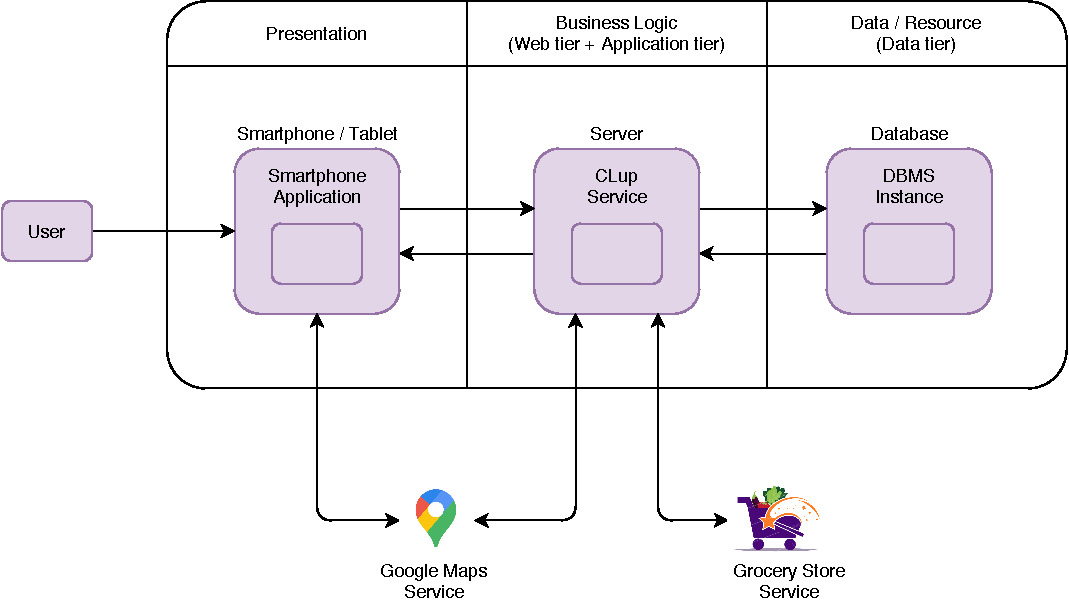
\includegraphics[width=1.0\textwidth]{images/architecture.pdf}
	\caption{System architecture.}
\end{figure}

\section{Component View}

\begin{sidewaysfigure}
	\centering
	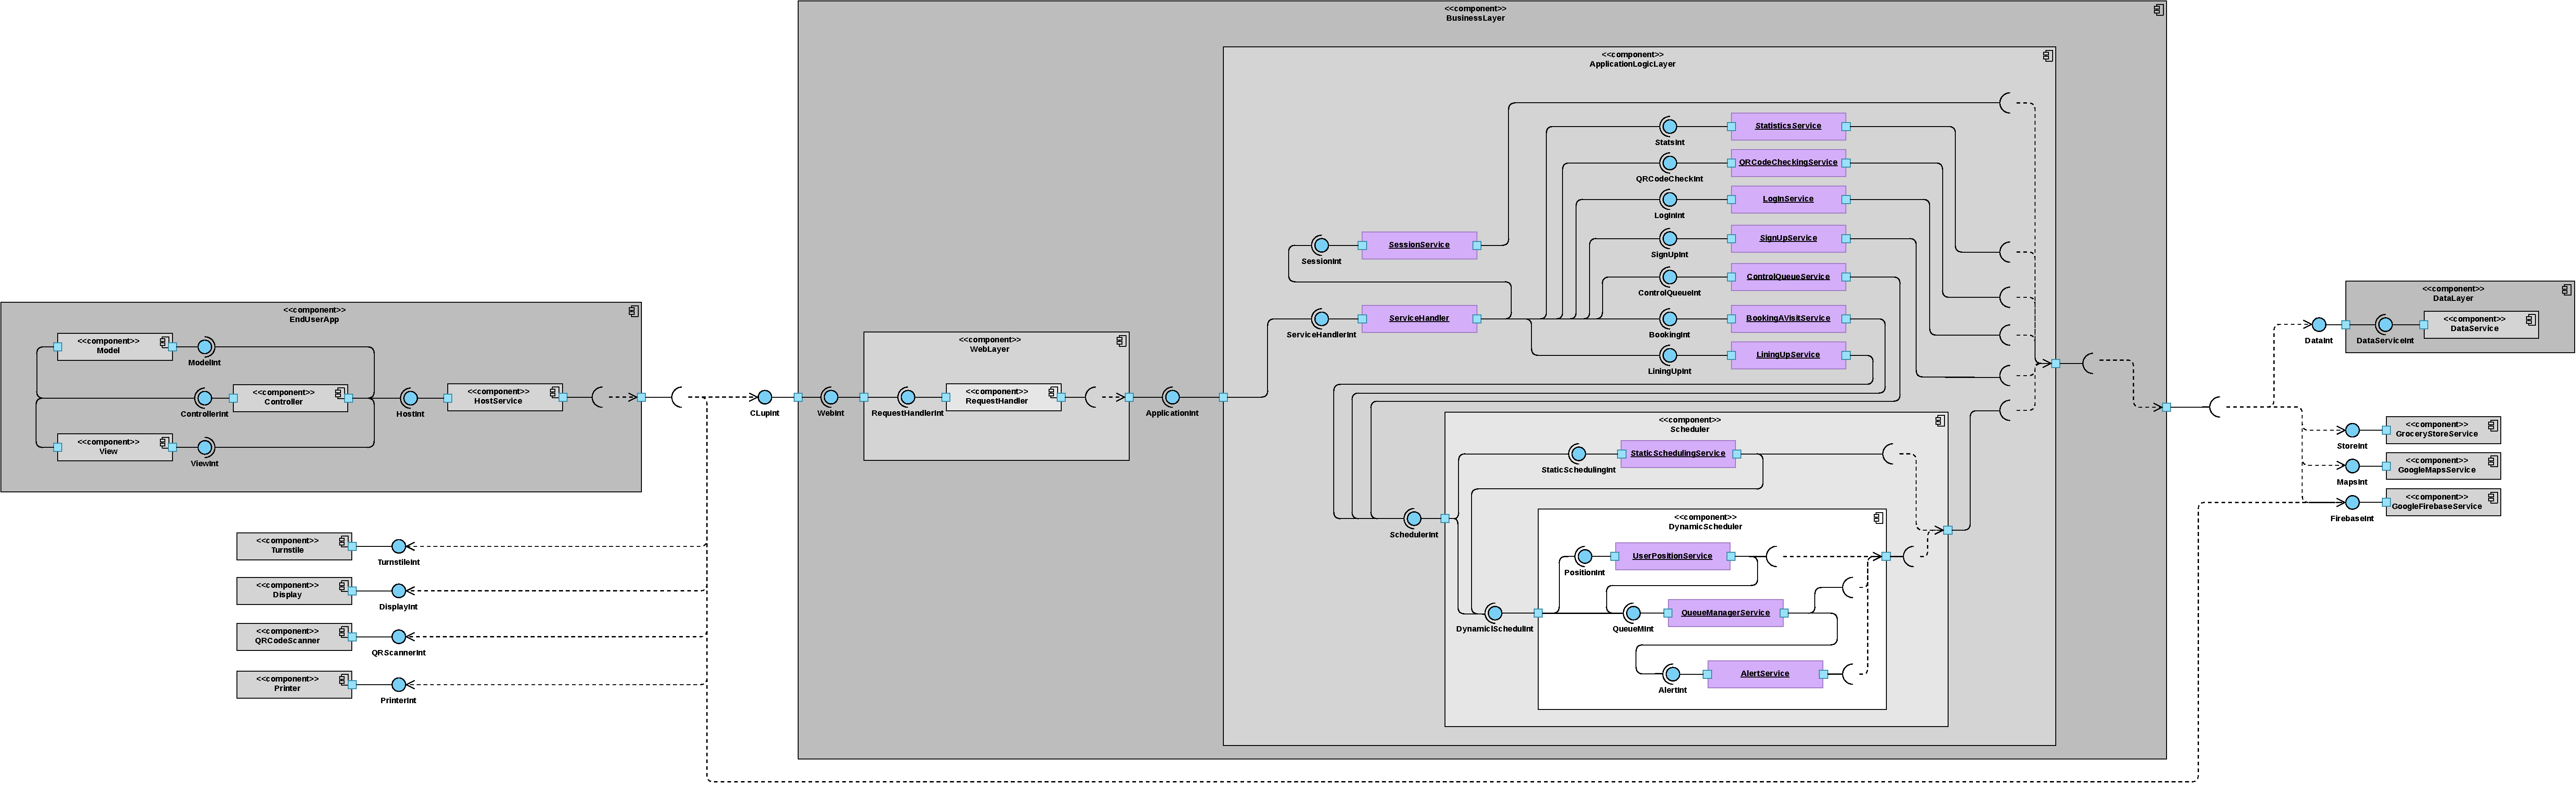
\includegraphics[width=1.0\textwidth]{images/component_diagram.pdf}
	\caption{Component Diagram.}
\end{sidewaysfigure}

\section{Deployment View}

\section{Runtime View}

\section{Component Interfaces}

\section{Selected Architectural Styles and Patterns}

\begin{figure}[H] % \begin{sidewaysfigure}
	\centering
	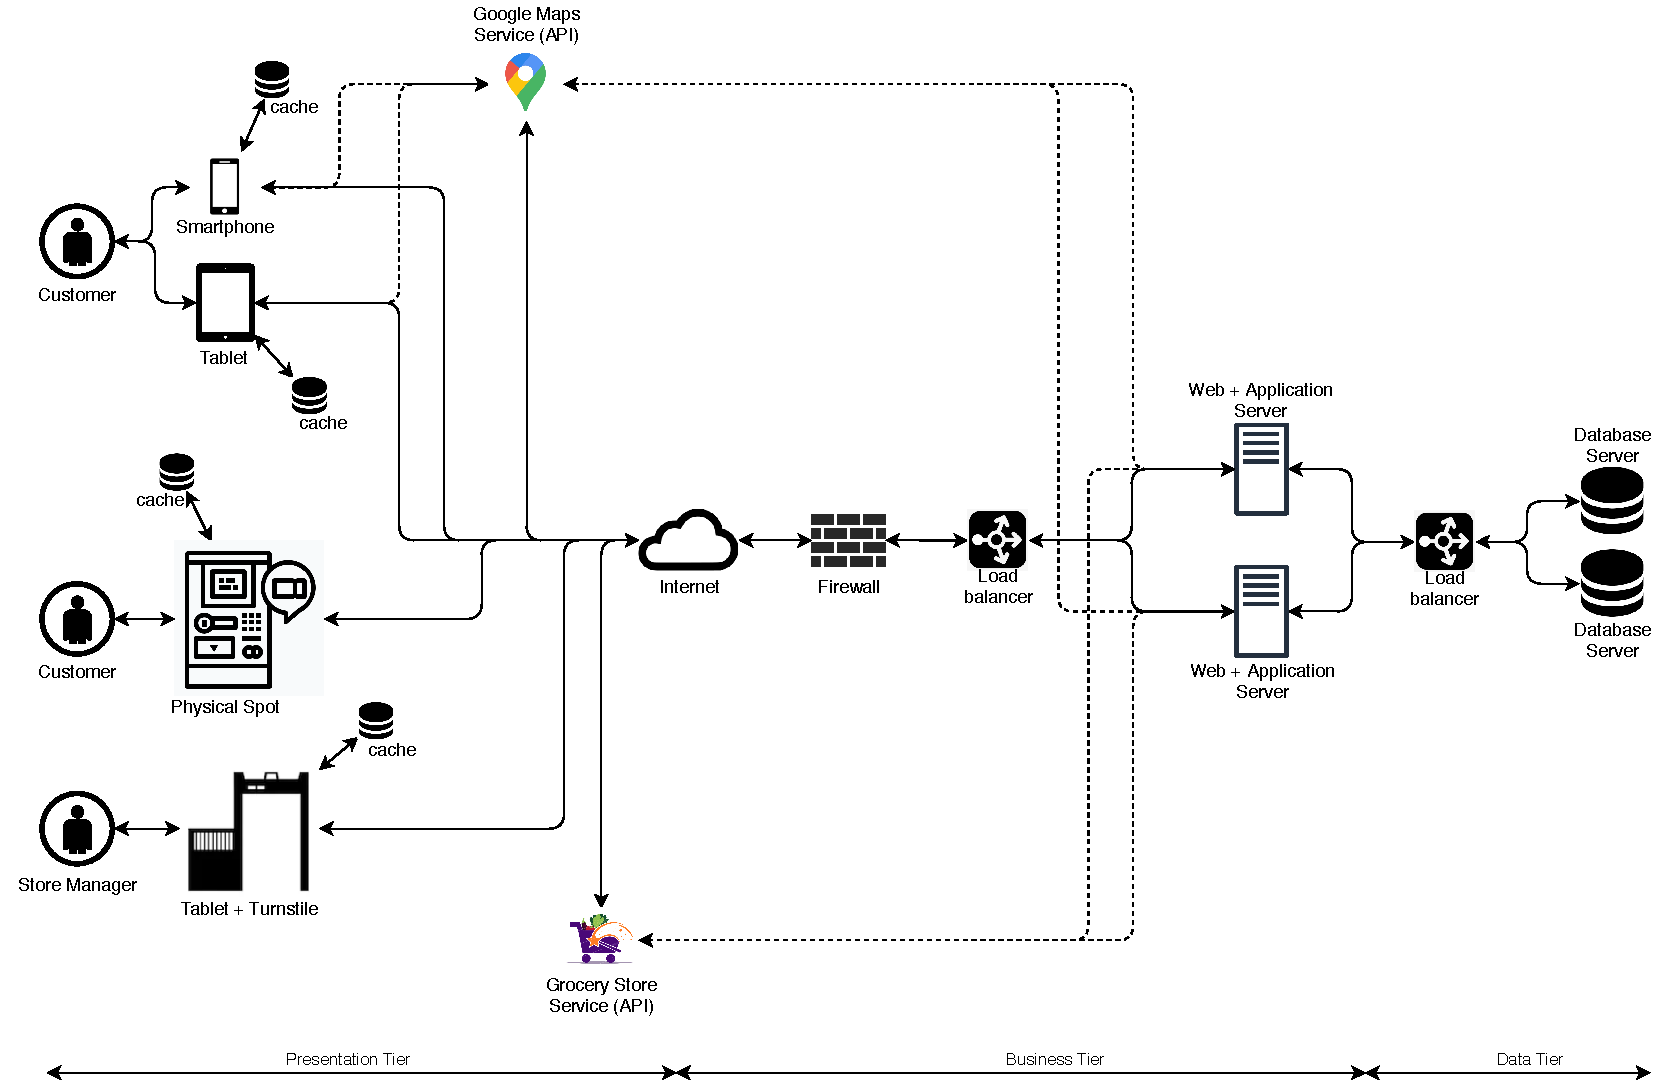
\includegraphics[width=1.0\textwidth]{images/architecture_components.pdf}
	\caption{Architecture components.}
\end{figure} % \end{sidewaysfigure}

\section{Other Design Decisions}
\chapter{User Interface Design}

Different mock-ups of the application have been shown in the \gls{rasd}.
In the current document we are going to present the \gls{ux} diagram~\ref{fig:UXDiagram} to help the reader in the understanding of the sequence of events and the relations between interfaces.

\begin{figure}[H]
	\centering
	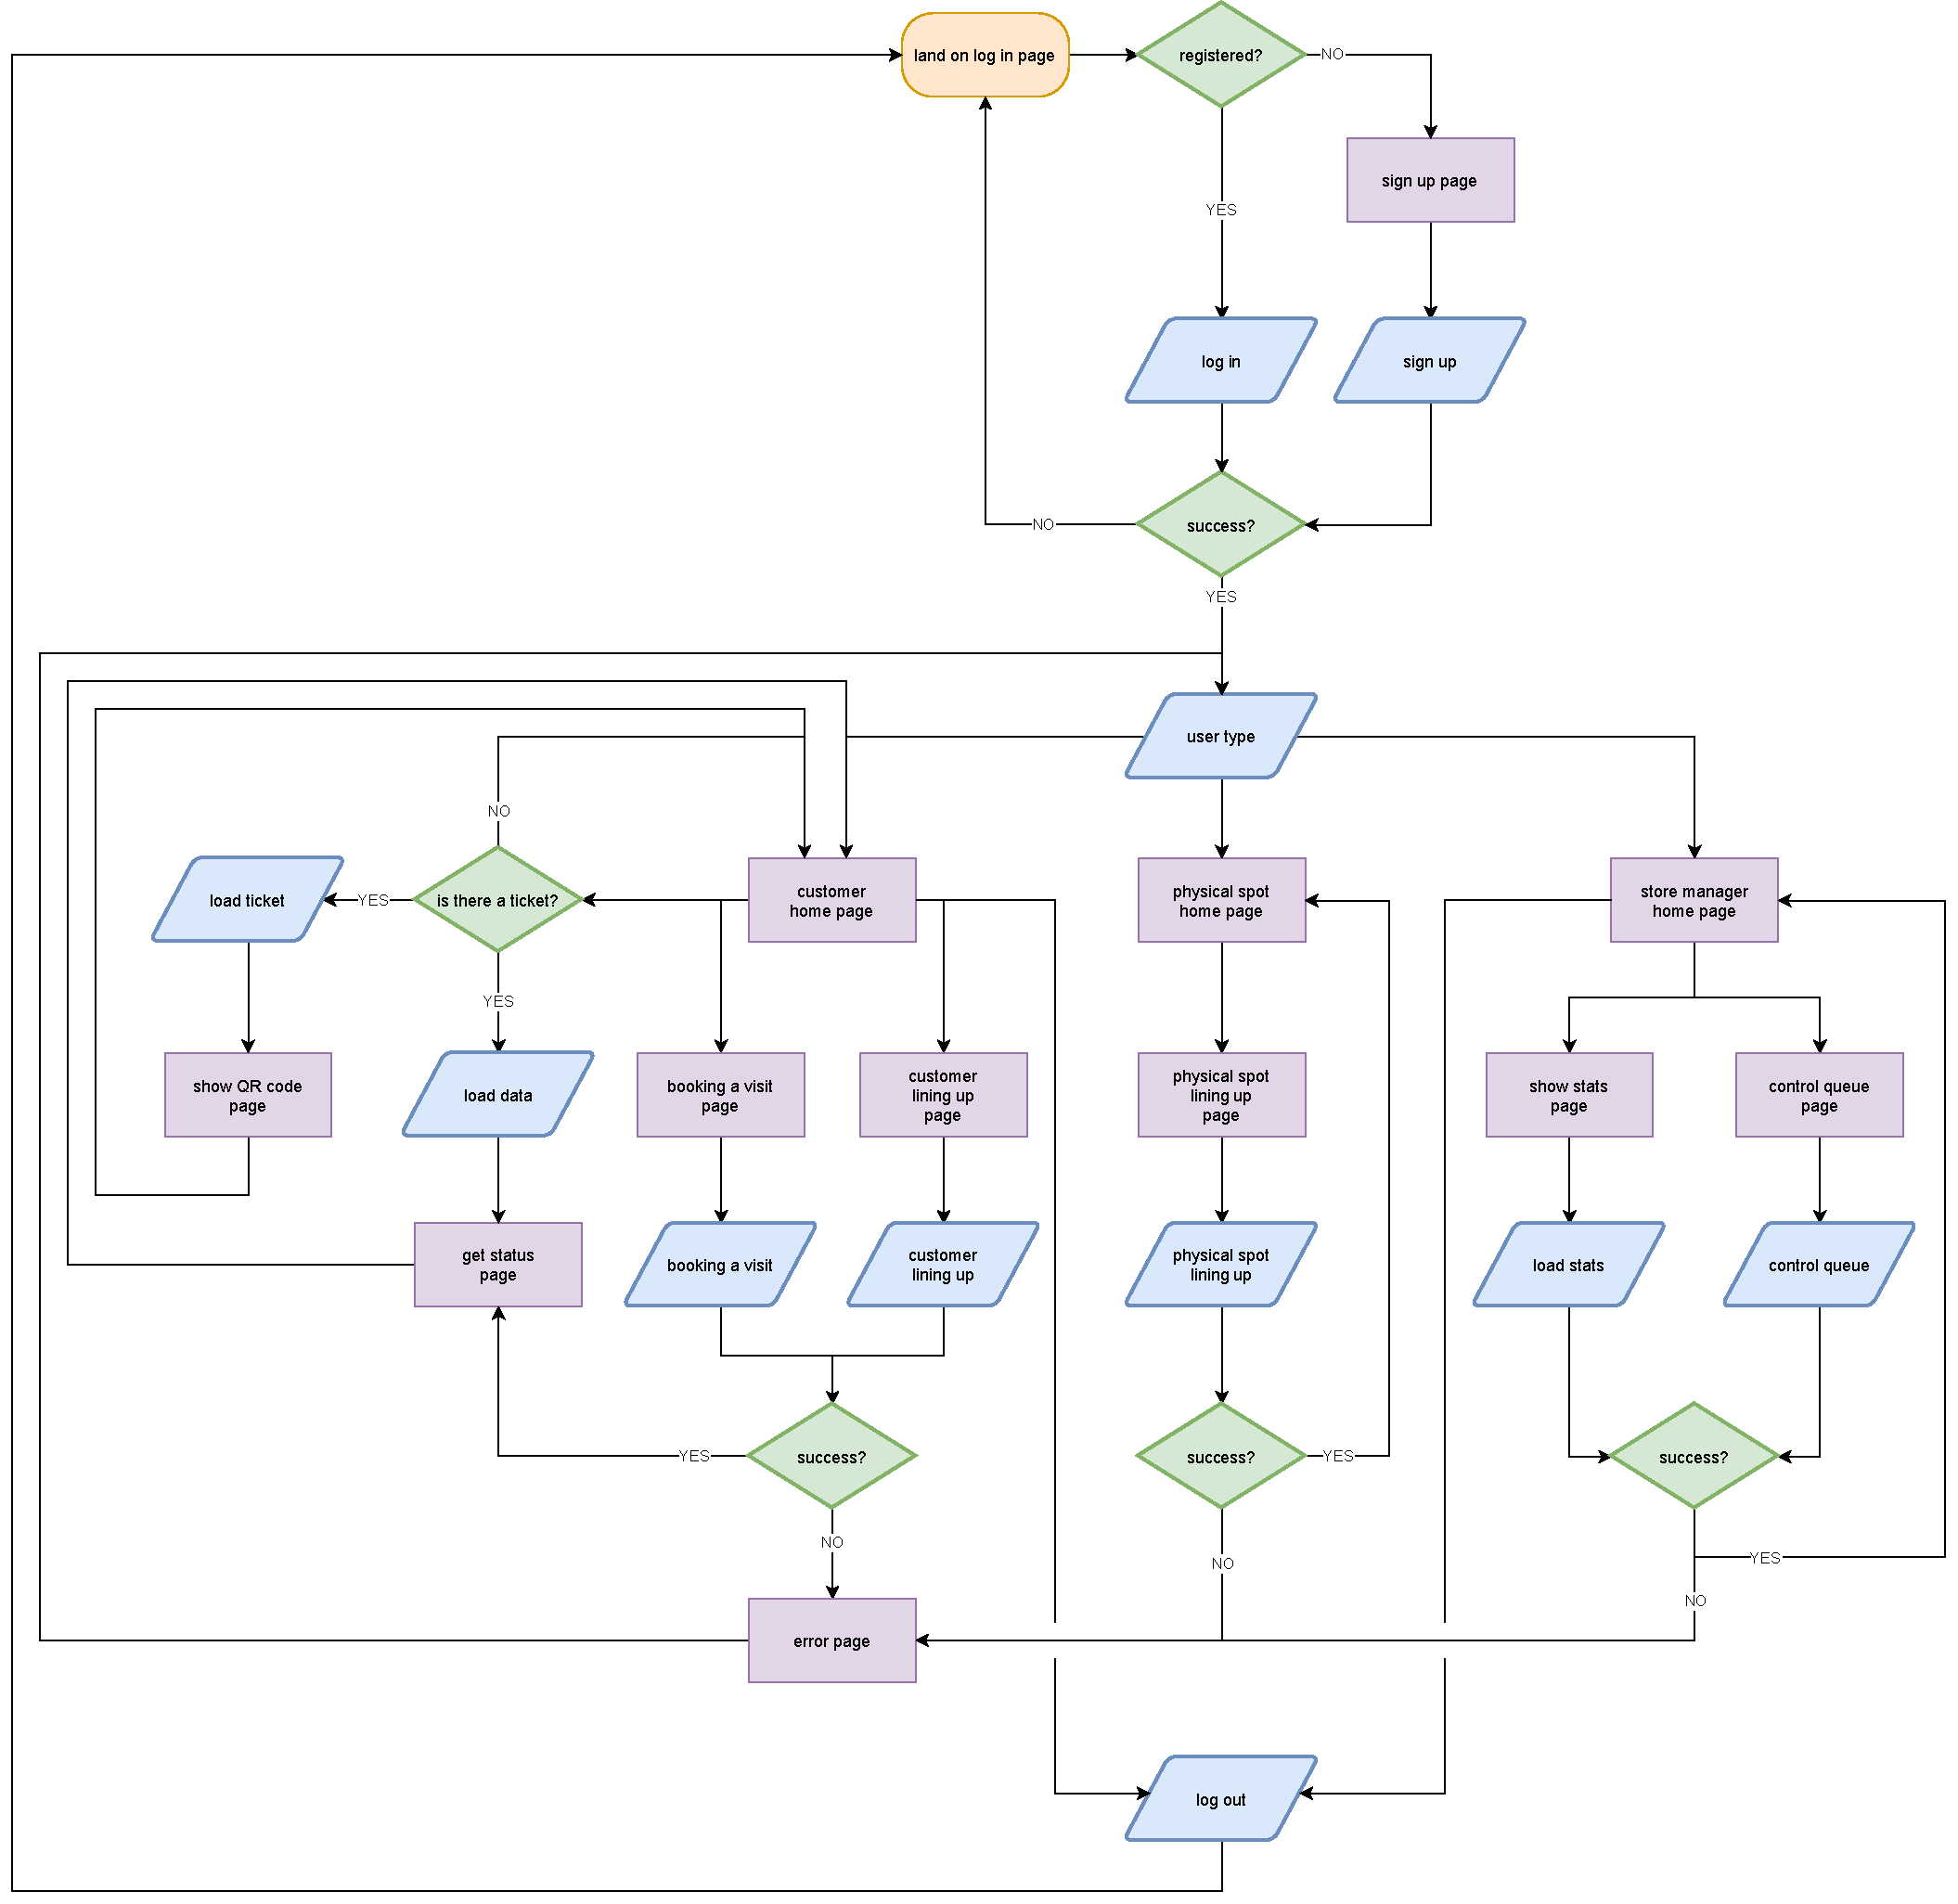
\includegraphics[width=0.9\textwidth]{images/UX.pdf}
	\caption{\gls{ux} diagram. \textit{Yellow} boxes represent \textbf{start}ing and \textbf{end}ing \textbf{points}. \textit{Green} boxes are for \textbf{decisions}. \textit{Violet} boxes are for \textbf{processes}. \textit{Blue} boxes are for \textbf{inputs/outputs}.}\label{fig:UXDiagram}
\end{figure}


\chapter{Requirements Traceability}
\begin{itemize}

	\item {\textbf{[R1]}}: The system has to schedule entrances to the store.\\
	component:
	\begin{itemize}
	\item Scheduler
	\end{itemize}
	\item {\textbf{[R2]}}: The system has to compute the maximum capacity of the store w.r.t. the social distances imposed by the \gls{dpcm} in force.\\
	component:
	\begin{itemize}
	\item DataService
	\item StatisticService
	\end{itemize}
	\item {\textbf{[R3]}}: The system has to monitor the customers residence time in the store.
component:
	\begin{itemize}
	\item DataService 
	\item GroceryStoreService
	\end{itemize}
	\item {\textbf{[R4]}}: The system has to allow authorized customers to enter in the store.
component:
	\begin{itemize}
	\item DataService 
	\item QRCheckingService
	\item LiningUpService
	\item BookingService
	\item EndUserApp
	\end{itemize}
	\item {\textbf{[R5]}}: The system has to deny unauthorized customers to enter in the store.
component:
	\begin{itemize}
	\item DataService
	\item QRCheckingService
	\end{itemize}
	\item {\textbf{[R6]}}: The system has to know when a customer enters in the store.
component:
	\begin{itemize}
	\item DataService 
	\item QRCheckingService
	\end{itemize}
	\item {\textbf{[R7]}}: The system has to know when a customer has left the store.
component:
	\begin{itemize}
	\item DataService 
	\item GroceryStoreService
	\end{itemize}
	\item {\textbf{[R8]}}: The system has to estimate the residence time, of a customer, in the store.
component:
	\begin{itemize}
	\item DataService 
	\item StaticSchedulingService 
	\item QueueManagerService 
	\end{itemize}
	\item {\textbf{[R9]}}: The system has to infer the residence time of the customers based on past purchases.
component:
	\begin{itemize}
	\item DataService 
	\item GroceryStoreService 
	\item StaticSchedulingService
	\item QueueManagerService 
	\end{itemize}
	\item {\textbf{[R10]}}: The system has to estimate the time needed to arrive, to the store, from the position of the customer.
component:
	\begin{itemize}
	\item UserPositionService 
	\item GoogleMapsService 
	\end{itemize}
	\item {\textbf{[R11]}}: The system has to track the global position of the customers.
component:
	\begin{itemize}
	\item UserPositionService 
	\item GoogleMapsService
	\end{itemize}
	\item {\textbf{[R12]}}: The system has to release QR codes to the customers.
component:
	\begin{itemize}
	\item DataService 
	\item LiningUpService 
	\item BookingAVisitService  
	\item EndUserApp 
	\end{itemize}
	\item {\textbf{[R13]}}: The system has to allow store managers to limit the number of QR codes released.
component:
	\begin{itemize}
	\item Dataservice 
	\item ControlQueueService 
	\item EndUSerApp 
	\end{itemize}
	\item {\textbf{[R14]}}: The system has to allow the store manager to monitor the status of the queue.
component:
	\begin{itemize}
	\item Dataservice 
	\item ControlQueueService 
	\item EndUSerApp 
	\end{itemize}
	\item {\textbf{[R15]}}: The system has to notify customers about the remaining time to be authorized to enter in the store.
component:
	\begin{itemize}
	\item QueueManagerService  
	\item AlertService  
	\item GoogleFirebaseService 
	\end{itemize}
	\item {\textbf{[R16]}}: The system has to communicate which is the next served QR code number.
component:
	\begin{itemize}
	\item EndUserApp 
	\item statisticService
	\end{itemize}
	\item {\textbf{[R17]}}: The system has to allow customers to register to the application.
component:
	\begin{itemize}
	\item DataService 
	\item SingUpService
	\item EndUserApp  
	\end{itemize}
	\item {\textbf{[R18]}}: The system has to allow users to login to the application.
component:
	\begin{itemize}
	\item DataService 
	\item LoginService 
	\item EndUserApp  
	\end{itemize}
	\item {\textbf{[R19]}}: The system has to release QR codes to the customers through the application.
component:
	\begin{itemize}
	\item DataService 
	\item LiningUpService 
	\item BookingAVisitService 
	\item EndUserApp
	\end{itemize}
	\item {\textbf{[R20]}}: The system has to alert customers if the queue is full.
component:
	\begin{itemize}
	\item EndUserApp 
	\item LiningUpService 
	\item StaticSchedulingService
	\end{itemize}
	\item {\textbf{[R21]}}: The system has to encode the ticket number in the QR code.
component:
	\begin{itemize}
	\item LiningUpService
	\end{itemize}
	\item {\textbf{[R22]}}: The system has to allow customers to watch the QR code from the application.
component:
	\begin{itemize}
	\item EndUserApp 
	\item LiningUpService
	\end{itemize}
	\item {\textbf{[R23]}}: The system has to allow customers to watch the ticket number encoded in the QR code.
component:
	\begin{itemize}
	\item EndUserApp 
	\item LiningUpService
	\end{itemize}
	\item {\textbf{[R24]}}: The system has to allow customers to watch the remaining time to be authorized to enter in the store.
component:
	\begin{itemize}
	\item EndUserApp 
	\item LiningUpService
	\end{itemize}
	\item {\textbf{[R25]}}: The system has to update the remaining time showed to the customers.
component:
	\begin{itemize}
	\item QueueManager 
	\item LiningUpService
	\end{itemize}
	\item {\textbf{[R26]}}: The system has to allow customers to delete a ticket.
component:
	\begin{itemize}
	\item EndUserApp 
	\item LiningUpService
	\item BookingAVisitService  
	\end{itemize}
	\item {\textbf{[R27]}}: The system has to notify customers about the validation status of the QR code.
component:
	\begin{itemize}
	\item QueueManagerService 
	\item AlertService 
	\item GoogleFirebaseService   
	\end{itemize}
	\item {\textbf{[R28]}}: The system has to check if users have Internet connection active.
component:
	\begin{itemize}
	\item EndUserApp
	\end{itemize}
	\item {\textbf{[R29]}}: The system has to check if users have allowed the permissions requested by the application.
component:
	\begin{itemize}
	\item EndUserApp
	\end{itemize}
	\item {\textbf{[R30]}}: The system has to register store managers in the application.
component:
	\begin{itemize}
	\item DataService 
	\end{itemize}
	\item {\textbf{[R31]}}: The system has to allow store managers to monitor the number of customers inside the store.
component:
	\begin{itemize}
	\item EndUserApp 
	\item StatisticService 
	\item ControlQueueService 
	\end{itemize}
	\item {\textbf{[R32]}}: The system has to scan the QR codes of the customers.
component:
	\begin{itemize}
	\item QRCodeCheckingService
	\end{itemize}
	\item {\textbf{[R33]}}: The system has to allow store managers to modify the timing parameters of the scheduler.
component:
	\begin{itemize}
	\item DataService 
	\item StaticsService 
	\item EndUserApp 
	\end{itemize}
	\item {\textbf{[R34]}}: The system has to allow unregistered customers to line up.
component:
	\begin{itemize}
	\item EndUserApp 
	\item LiningUpService
	\end{itemize}
	\item {\textbf{[R35]}}: The system has to release QR codes from a physical spot.
component:
	\begin{itemize}
	\item DataService 
	\item LiningUpService 
	\item EndUserApp 
	\end{itemize}
	\item {\textbf{[R36]}}: The system has to print QR codes on a paper tickets.
component:
	\begin{itemize}
	\item LiningUpService
	\end{itemize}
	\item {\textbf{[R37]}}: The system has to alert when the paper and toner of the physical spot is going to finish.
component:
	\begin{itemize}
	\item LiningUpService
	\end{itemize}
	\item {\textbf{[R38]}}: The system has to allow customers to specify the date and time for a visit to the store.
component:
	\begin{itemize}
	\item EndUserApp
	\end{itemize}
	\item {\textbf{[R39]}}: The system has to allow customers to specify the category of grocery they want to buy.
component:
	\begin{itemize}
	\item EndUserApp
	\end{itemize}

\end{itemize}
\chapter{Implementation, Integration and Test Plan}
\section{Overview}
In this section we will focus on steps to be conducted for the implementation, integration and test plan. 
Firstly, we ensure all the single units are created and tested on their own. Then we combine these unary modules into clusters that will perform a specific software sub-function. This will allow us to start the integrated testing of this clusters and test the interfaces between the units. This is crucial since the logic implemented in the modules differ from developer to developer. So, by testing them we ensure they work properly, and in case it allows us to detect possible errors in the interfaces. This process is repeated clustering the new formed units, until we reach the end.
The software integration test is to be repeated again several times to ensures that no new previously undetected errors spawn. It serves also to ensure that the correct performance level is reached.

\section{Integration testing approach:}
The approach chosen to the integration testing is the bottom-up one. It starts testing from the lowest unit of the application and gradually moves towards integrating and testing the upper ones until all the units are integrated as one. Then the system as whole is tested. This process require the use of drivers that are disposable components made ad hoc to be placed on a higher level of the component tested to call their function. 
This approach was chosen because it allows us to localize in an easier way the possible errors in the lower levels, where is present the most complex component, the scheduler. The approach divides the component in five ordered blocks.\\

\begin{figure}[H]
    \centering
    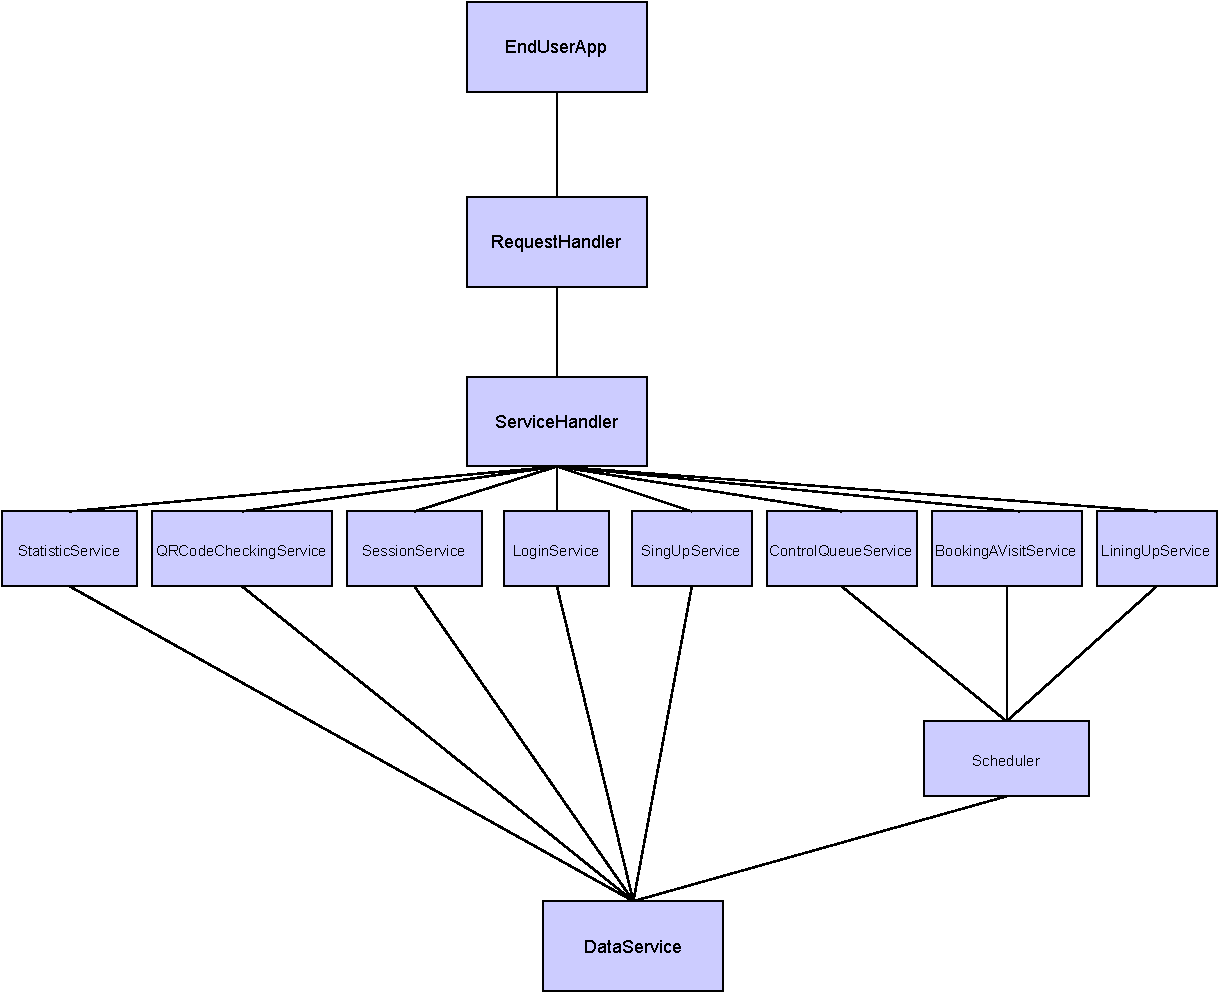
\includegraphics[width=1.0\textwidth]{images/component_hierarchy.pdf}
    \caption{hierarchy of components.}
\end{figure}

As shown in the hierarchy of the components, the lowest component of the system and so the first one to be tested and implemented is the DataService. Every other component directly or not, rely on this one since they require to store and retrieve data to function. On the other hand, the data service does not rely on other components and so it can function in isolation. \\
The Scheduler should be implemented next and so as second block, since it is the most complex system of the bottom level ones that use different component to function. Its function is to schedule both statically and dynamically for the app users, the order of their turn in the queue. It requires to consider both people that lined up and booked a visit, and possibly their data and position. It also ineteracts through the FireBaseService with the app-users to notify them when it is their turn.
Inside the scheduler the first component to be implemented is the StaticSchedulingService. Since it is the one that handles first the request from the higher level and could function independently of the DynamicScheduler. It requires to build the drivers of the basic function of the upper modules and the integration with GoogleMapsServices and GroceryStoreService. After that the DynamicScheduler has to be implemented starting from the AlertService and a drive of the QueueManager to verify that the notification request are sent correctly to the GoogleFireBaseService. Then QueueManagerService and UserPositionService can be implemented and integrated in parallel. \\
The third block commence after the start of the implementation of the scheduler, the component to be integrated in parallel or immediately following are the StatisticService, QRCodeCheckingSerivice, LoginService, SingUpService and SessionService. Since all of them work independently to each other their order is also interchangeable, but the order of implementation chosen is the following:
The first one is StatisticService, it offers function to the store manager and it is not strictly bond with the client interface. The second and third are LoginService and SingUpService, one serves to allow user to login and the other to allow user to sign in. The fourth one checks that the information scanned by the turnstile are correct and match the ones in the database. The last one, SessionService manages the session of the different users and so it more dependent on the higher levels. All of them require the use and so the develop of a driver of the ServiceHandler. \\
Subsequently the fourth block begin, after the scheduler is integrated, the component to implements are ControlQueueService, BookingAVisitService and LiningUpService. All of them need a driver for the ServiceHandler and must interact with the scheduler. The first one to change parameters and block the release of the new tickets, the second and third ones allow user to get respectively booking ticket and lining up ticket. The BookingAVisitService permits also to insert more information about the visit while the LiningUpService has also to check the user type to decide to monitor their position. The order of implementation of this block of component is the following: First the LiningUpService since it is the most important of the three then BookingAVisitService and lastly the ControlQueueService because it will be easier to check if it works as expected if the LiningUpService is already implemented. \\
And in the end the last block to be integrated is composed in order of the ServiceHandler, RequestHandler and the EndUserApp. The order of integration is clear since they are in different levels, it require to develop the RequestHandler and then EndUserApp drivers when proceeding on the implementation. 
Since they are the last ones to be implemented the testing should be done more meticulously to ensure that the almost complete system works as thought. Especially because these components are crucial to its functioning, they allow so send the request from the device, elaborate them and redirect on the right component.\\
The interfaces of the hardware component of the store and so turnstile, scanner and printer are included in the GroceryStoreSerivice. And so even though they are already implemented and tested, they should by further tested on site to verify that the acquisition of data, the output data and the state transition are correct. 
\begin{figure}[H]
    \centering
    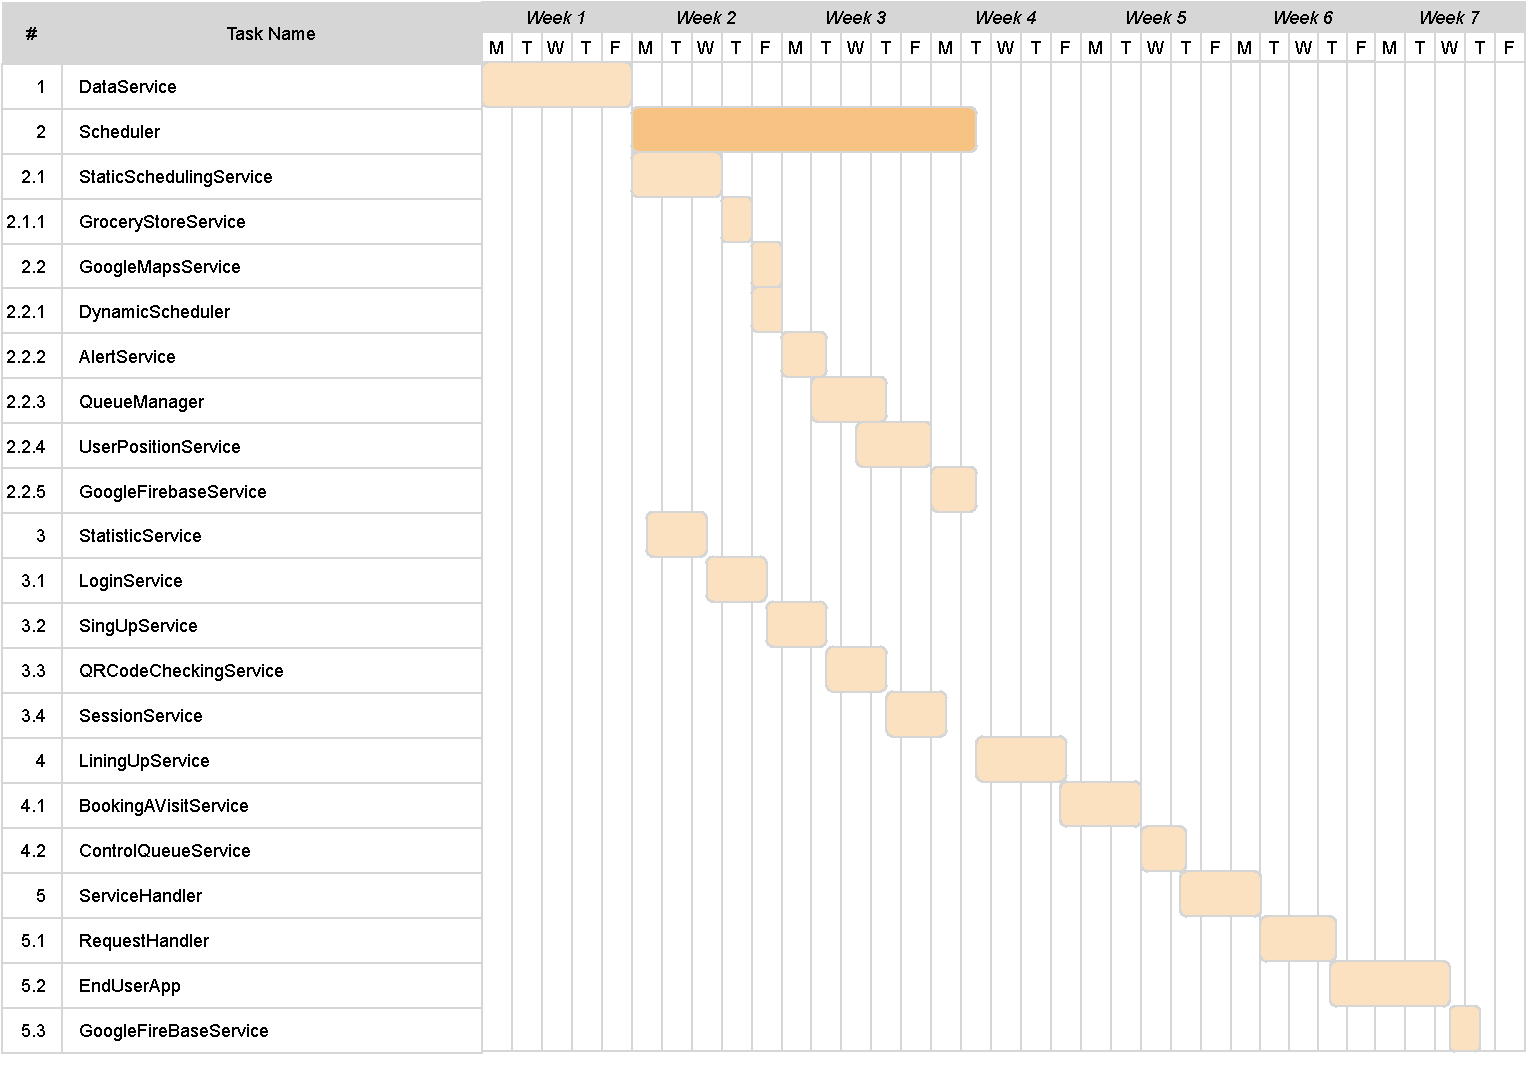
\includegraphics[width=1.0\textwidth]{images/Gantt.pdf}
    \caption{Gantt chart.}
\end{figure}

\section{Integration strategy :}
As stated in the previous section,the approach chosen it the bottom-up one so the first component to be unit tested is the DataService. After it is implemented on top of that the scheduler and a driver to simulate the inputs.
\begin{figure}[H]
    \centering
    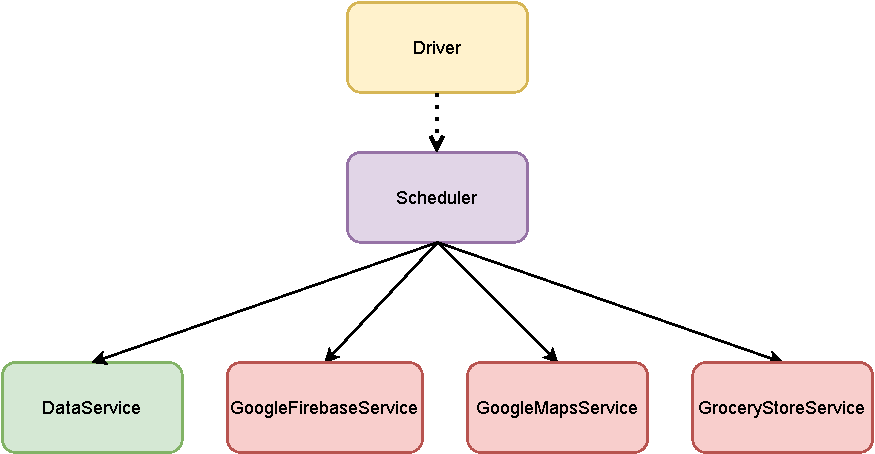
\includegraphics[width=1.0\textwidth]{images/component1.pdf}
    \caption{Integration step 1.}
\end{figure}
The scheduler being a complex component includes first the implementation of the StaticSchedulingService with the DataService and the two external services. Next the AlertService has to be implemented with GoogleFirebaseService
\begin{figure}[H]
    \centering
    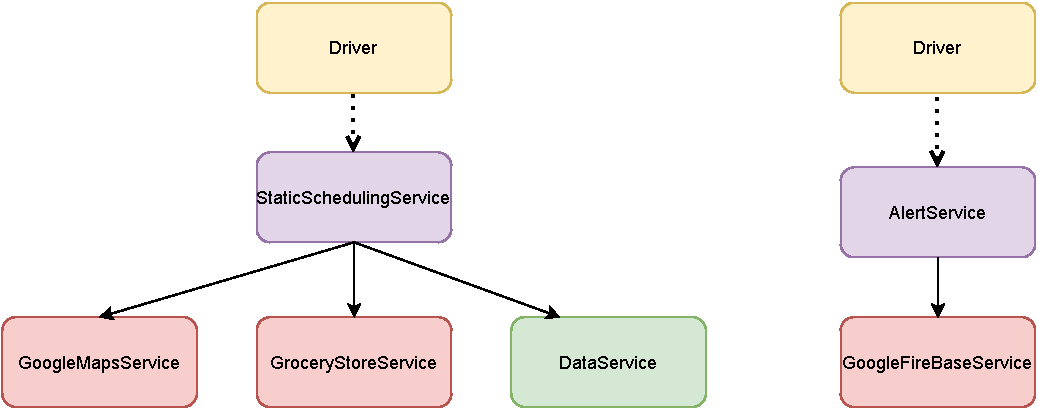
\includegraphics[width=1.0\textwidth]{images/component2.pdf}
    \caption{Integration step 2.}
\end{figure}
Then the QueueManagerService is implemented and integrated with the StaticSchedulingService and AlertService. Which causes the merge of the two small clusters.
\begin{figure}[H]
    \centering
    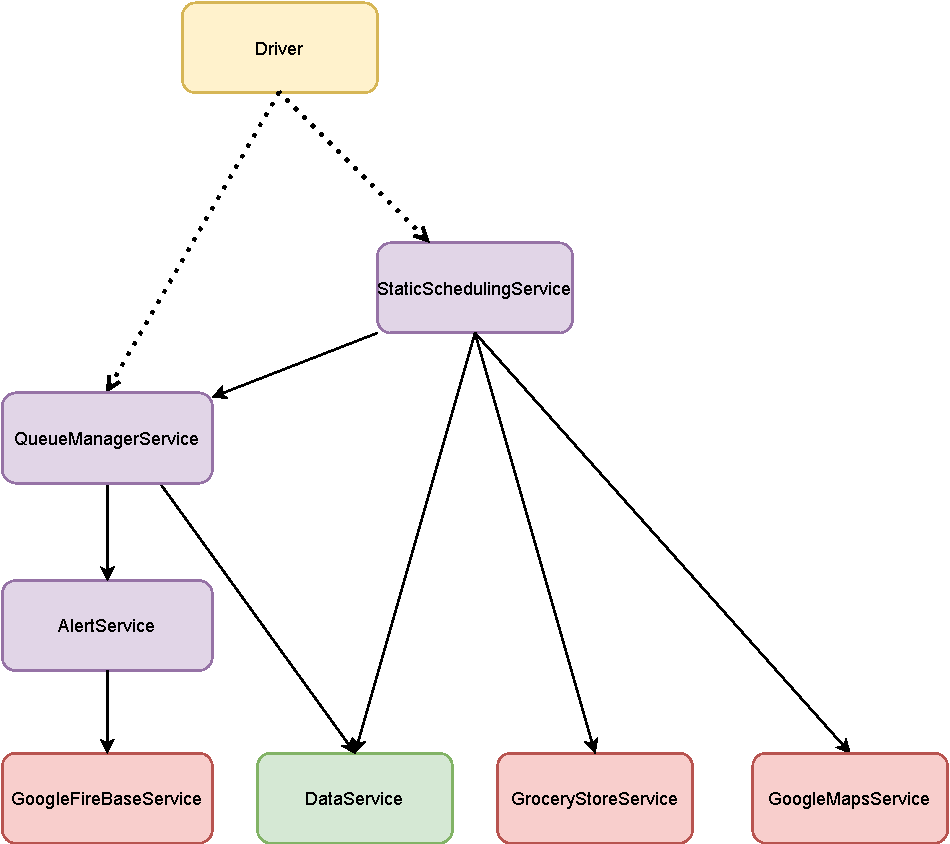
\includegraphics[width=1.0\textwidth]{images/component3.pdf}
    \caption{Integration step 3.}
\end{figure}
The UserPositionSerivice is implemented for last inside the scheduler and it completes it.
\begin{figure}[H]
    \centering
    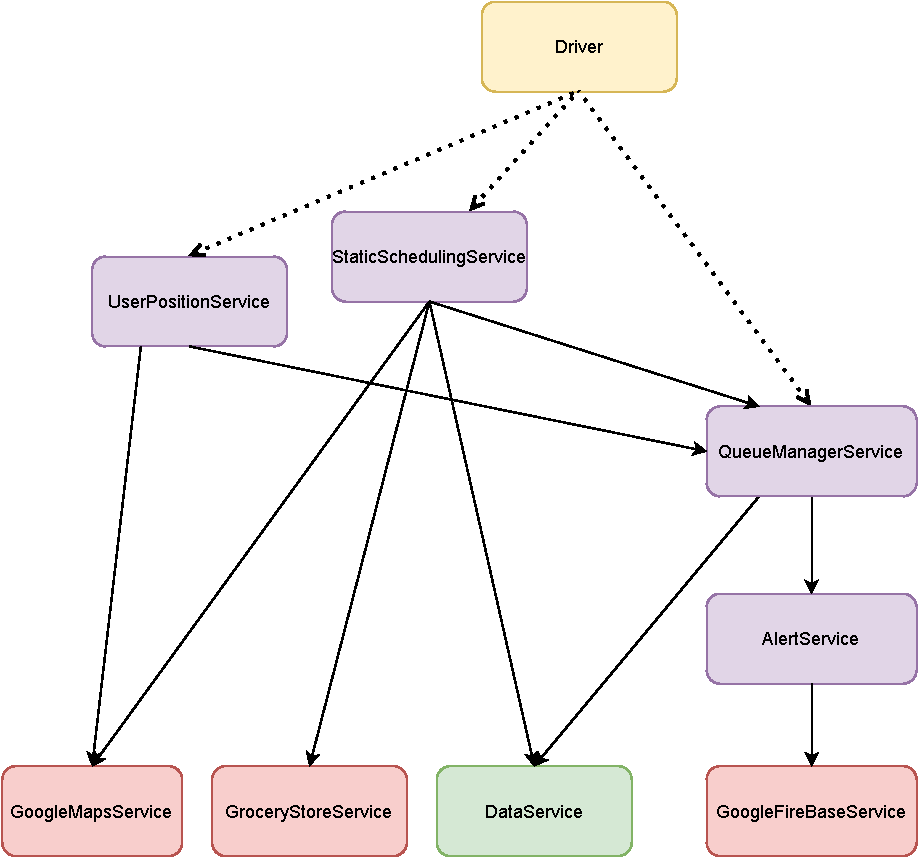
\includegraphics[width=1.0\textwidth]{images/component4.pdf}
    \caption{Integration step 4.}
\end{figure}
Simultaneously the components StatisticService, LoginService, SignUpService, QRCodeCheckingService and SessionService are implemented on the DataService in this order,with a driver of the ServiceHandler.
\begin{figure}[H]
    \centering
    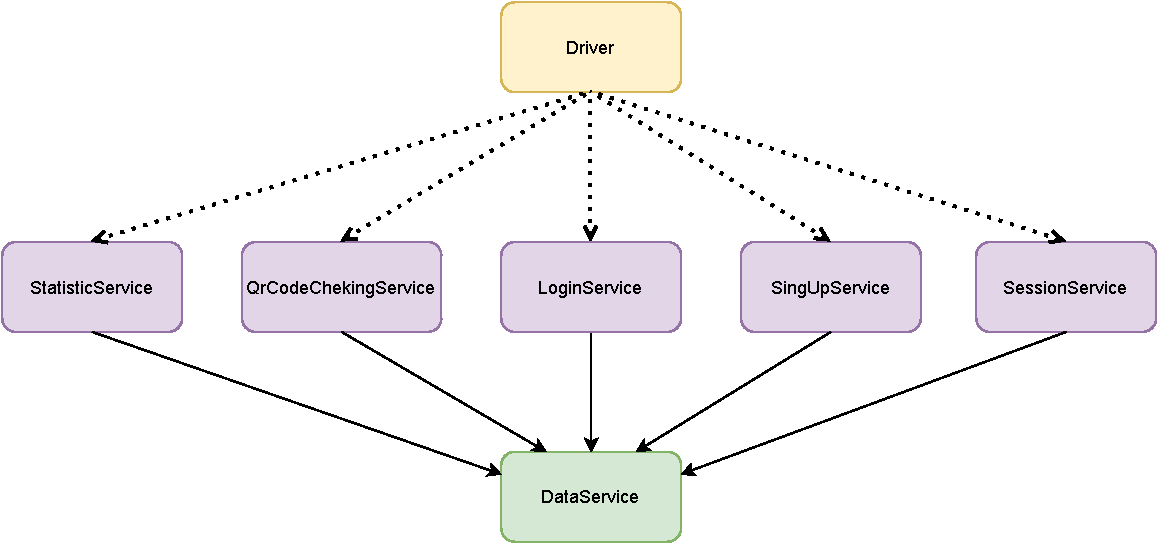
\includegraphics[width=1.0\textwidth]{images/component5.pdf}
    \caption{Integration step 5.}
\end{figure}
After the integration of the scheduler, the components that are implemented on top are in order LiningUpService, BookingAVisitService, ControlQueueService.
\begin{figure}[H]
    \centering
    \includegraphics[width=1.0\textwidth]{images/component6.pdf}
    \caption{Integration step 6.}
\end{figure}
Lastly, the component implemented are the ServiceHandler with the driver on top, then the RequestHandler with the driver and finally the EndUserApp with the GoogleFirebaseService.
\begin{figure}[H]
    \centering
    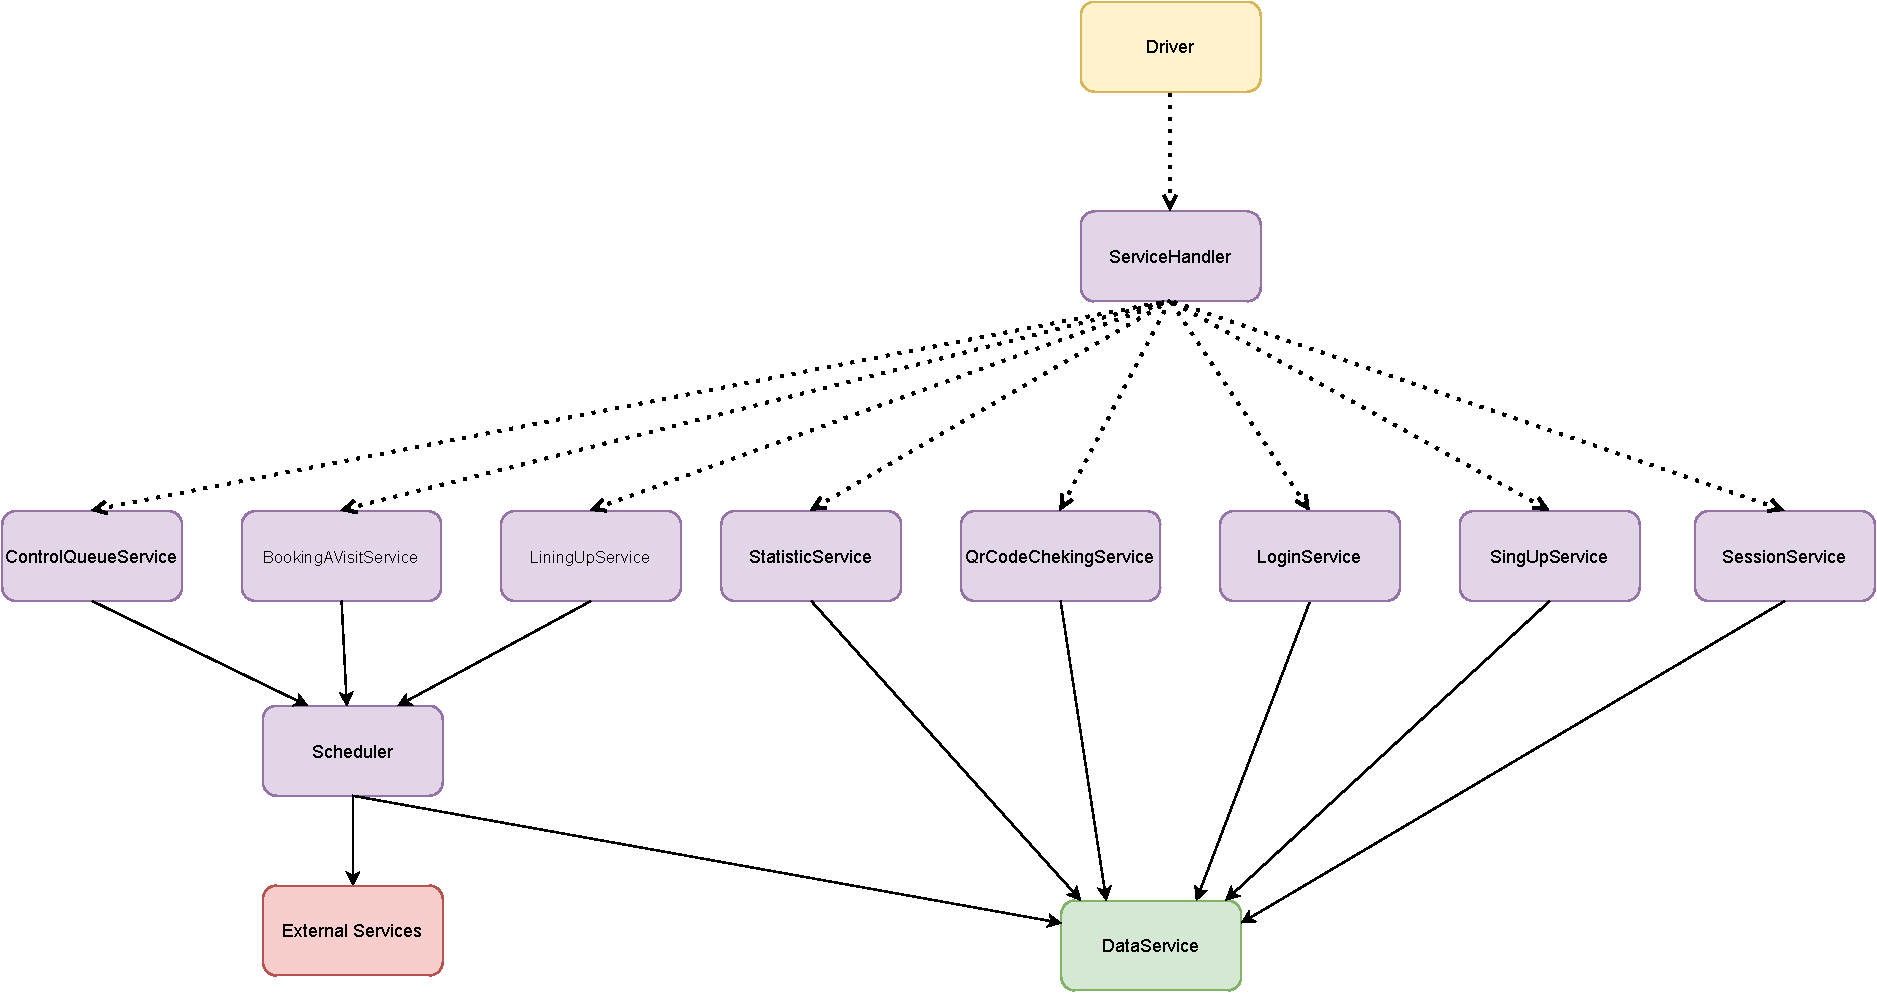
\includegraphics[width=1.0\textwidth]{images/component7.pdf}
    \caption{Integration step 7.}
\end{figure}
\begin{figure}[H]
    \centering
    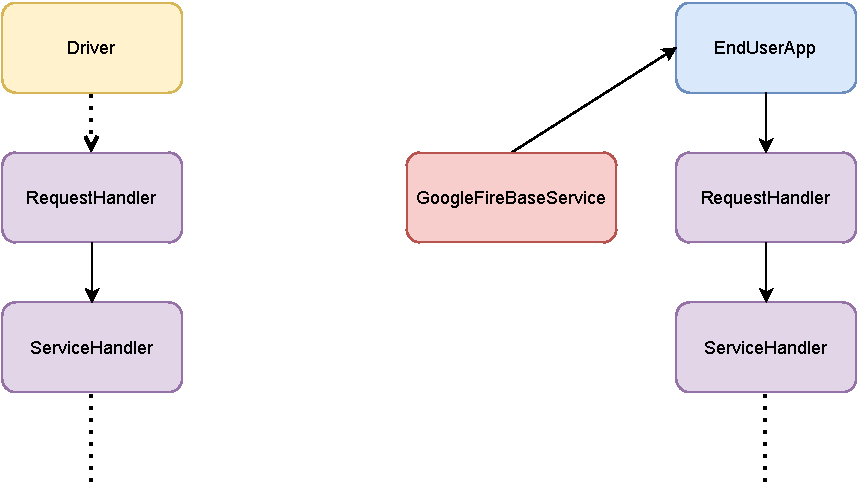
\includegraphics[width=1.0\textwidth]{images/component8.pdf}
    \caption{Integration step 8.}
\end{figure}

\chapter{Effort Spent}

\begin{table}[H]
    \centering
    \begin{tabular}{| m{0.8\textwidth} | m{0.2\textwidth} |}
        \hline
        \textbf{Topic}                                                             & \textbf{Hours} \\
        \hline
        Preliminary Discussion                                                     & 6              \\
        \hline
        Introduction                                                               & 4              \\
        \hline
        Product Perspective                                                        & 6              \\
        \hline
        Product Functions                                                          & 1              \\
        \hline
        User Characteristics                                                       & 2              \\
        \hline
        Assumptions, Dependencies and Constraints                                  & 1              \\
        \hline
        External Interface Requirements                                            & 2              \\
        \hline
        Functional Requirements                                                    & 5              \\
        \hline
        Performance Requirements / Design Constraints / Software System Attributes & 5              \\
        \hline
        Alloy Code                                                                 & 12             \\
        \hline
        Revision                                                                   & 4              \\
        \hline
        \hline
        \textbf{Total:}                                                            & 48             \\
        \hline
    \end{tabular}
    \caption{Effort spent by Jas Valencic.}
\end{table}

\begin{table}[H]
    \centering
    \begin{tabular}{| m{0.8\textwidth} | m{0.2\textwidth} |}
        \hline
        \textbf{Topic}                                                             & \textbf{Hours} \\
        \hline
        Preliminary Discussion                                                     & 6              \\
        \hline
        Introduction                                                               & 3              \\
        \hline
        Product Perspective                                                        & 3              \\
        \hline
        Product Functions                                                          & 3              \\
        \hline
        User Characteristics                                                       & 1              \\
        \hline
        Assumptions, Dependencies and Constraints                                  & 2              \\
        \hline
        External Interface Requirements                                            & 8              \\
        \hline
        Functional Requirements                                                    & 10             \\
        \hline
        Performance Requirements / Design Constraints / Software System Attributes & 3              \\
        \hline
        Alloy Code                                                                 & 5              \\
        \hline
        Revision                                                                   & 4              \\
        \hline
        \hline
        \textbf{Total:}                                                            & 48             \\
        \hline
    \end{tabular}
    \caption{Effort spent by Damiano Derin.}
\end{table}
\chapter{References}

\begin{itemize}
    \item Specification document: "R \& DD Assignment AY2020-2021.pdf".
    \item Slides of the lectures.
    \item \glspl{rasd} of past students.
    \item Alloy documentation: "http://alloy.mit.edu/alloy/documentation.html"
    \item Google Maps services: "https://cloud.google.com/maps-platform"
    \item Google Firebase service: "https://firebase.google.com/"
\end{itemize}

%\end{linenumbers}


% bibliogarphy should be moved under References!
%*******************************************************
% Bibliografia
%*******************************************************
\nocite{*}
\bibliography{bib/bibliography}
\bibliographystyle{plain}

%*******************************************************
% Glossario
%*******************************************************
\glsaddall
\printglossary[type=\acronymtype,title={Glossary}]

\end{document}
